% !TeX program = xelatex
\documentclass[UTF8,11pt,a4paper]{ctexart}

\usepackage[a4paper,margin=2.2cm,top=1.8cm,bottom=2.2cm]{geometry}
\usepackage{fontspec}
\usepackage{graphicx}
\usepackage{array}
\usepackage{booktabs}
\usepackage{tabularx}
\usepackage{multirow}
\usepackage{amsmath,amssymb,bm}
\usepackage[
  backend=biber,
  style=nature,
  autocite=superscript,
  sorting=none,
  maxbibnames=99,
  giveninits=true
]{biblatex}
\usepackage{caption}
\usepackage{subcaption}
\usepackage{enumitem}
\usepackage{algorithm}
\usepackage{algpseudocode}
\usepackage{titlesec}
\usepackage{fancyhdr}
\usepackage{xcolor}
\usepackage{hyperref}
\usepackage[nameinlink,noabbrev]{cleveref}
\usepackage{float}
\usepackage{setspace}
\usepackage{tikz}

% ---- template font rules ----
% Chinese text: SimSun (Songti) at the current template size.
% English text: Times New Roman.
% Journal masthead "SHIT": Arial Black to match the sample style.
\setmainfont{Times New Roman}
\setsansfont{Arial}
\setCJKmainfont[AutoFakeBold=2.8,AutoFakeSlant=0.2]{SimSun}
\newfontfamily\shitlogofont{Arial Black}
\graphicspath{{./fig/}}
\addbibresource{references.bib}

\hypersetup{colorlinks=true,linkcolor=blue,citecolor=blue,urlcolor=blue}
% Nature-style references: default citations are blue superscripts.
\let\inlinecite\cite
\let\inlineparencite\parencite
\let\cite\supercite
\let\parencite\supercite
\let\autocite\supercite
\AtEveryCitekey{\color{blue}}
\crefname{figure}{Fig.}{Figs.}
\Crefname{figure}{Fig.}{Figs.}
\crefname{table}{Table}{Tables}
\Crefname{table}{Table}{Tables}
\crefname{algorithm}{Algorithm}{Algorithms}
\Crefname{algorithm}{Algorithm}{Algorithms}
\crefname{equation}{Eq.}{Eqs.}
\Crefname{equation}{Eq.}{Eqs.}
\crefname{section}{Section}{Sections}
\Crefname{section}{Section}{Sections}
\setlength{\parindent}{2em}
\setlength{\parskip}{0pt}
\linespread{1.10}
\columnsep=0.75cm

\pagestyle{fancy}
\fancyhf{}
\renewcommand{\headrulewidth}{0.4pt}
\fancyhead[L]{\footnotesize\itshape \shorttitle}
\fancyhead[R]{\footnotesize SHIT / 构石}
\fancyfoot[C]{\thepage}

\titleformat{\section}{\bfseries\Large}{\thesection}{0.6em}{}
\titleformat{\subsection}{\bfseries\normalsize}{\thesubsection}{0.6em}{}
\titleformat{\subsubsection}{\bfseries\normalsize}{\thesubsubsection}{0.6em}{}
\titlespacing*{\section}{0pt}{1.0em}{0.5em}
\titlespacing*{\subsection}{0pt}{0.8em}{0.3em}
\titlespacing*{\subsubsection}{0pt}{0.6em}{0.2em}
\captionsetup{font=small,labelfont=bf}

% ---- metadata ----
\newcommand{\journalname}{SHIT}
\newcommand{\journalcname}{构石}
\newcommand{\journalsubtitle}{Sciences\\Humanities\\Information\\Technology}
\newcommand{\subjectsection}{Subject Section}
\newcommand{\papervolume}{YYYY}
\newcommand{\paperissue}{0--0}
\newcommand{\paperdoi}{没有 doi}
\newcommand{\advancepubdate}{DD Month YYYY}
\newcommand{\manuscriptcategory}{构石研究 / Interdisciplinary}
\newcommand{\associatededitor}{XXXXXXX}
\newcommand{\receiveddate}{XXXXX}
\newcommand{\reviseddate}{XXXXX}
\newcommand{\accepteddate}{XXXXX}
\newcommand{\shorttitle}{Article short title}
\newcommand{\shortauthors}{A. Author et al.}
\newcommand{\contactemail}{example@example.org}
\newcommand{\availabilitytext}{本文所用材料、代码与构石样本可按需联系通讯作者索取。}
\newcommand{\supplementarytext}{附录、补充证明与额外构石案例见补充材料。}
\newcommand{\aistatementtext}{请在此说明生成式人工智能工具的使用情况。建议参考如下格式填写：During the preparation of this work the author(s) used [tool or service name] for [purpose]. After using this tool or service, the author(s) reviewed and edited the content as needed and take full responsibility for the content of the publication. 若未使用生成式人工智能或 AI-assisted tools，可写“None”或明确声明未使用。}

\newcommand{\papertitle}{Manuscript Title（请用中文写）}
\newcommand{\paperauthors}{Corresponding Author$^{1,*}$, Co-author$^2$ and Co-author$^2$}
\newcommand{\paperaffiliations}{$^1$Department of XXXXXXX, Address XXXX etc., $^2$Department of XXXXXXX, Address XXXX etc.}

\newcommand{\motivationtext}{请用中文写。}
\newcommand{\resultstext}{请用中文写。}
\newcommand{\availabilityblock}{请用中文写。}
\newcommand{\supplementaryblock}{请用中文写。}

\newcommand{\settitleblock}[3]{\renewcommand{\papertitle}{#1}\renewcommand{\paperauthors}{#2}\renewcommand{\paperaffiliations}{#3}}
\newcommand{\setshorttitle}[1]{\renewcommand{\shorttitle}{#1}}
\newcommand{\setshortauthors}[1]{\renewcommand{\shortauthors}{#1}}
\newcommand{\setjournalmeta}[6]{\renewcommand{\papervolume}{#1}\renewcommand{\paperissue}{#2}\renewcommand{\paperdoi}{#3}\renewcommand{\advancepubdate}{#4}\renewcommand{\manuscriptcategory}{#5}\renewcommand{\associatededitor}{#6}}
\newcommand{\setdates}[3]{\renewcommand{\receiveddate}{#1}\renewcommand{\reviseddate}{#2}\renewcommand{\accepteddate}{#3}}
\newcommand{\setcontact}[3]{\renewcommand{\contactemail}{#1}\renewcommand{\availabilitytext}{#2}\renewcommand{\supplementarytext}{#3}}
\newcommand{\setabstractblocks}[4]{\renewcommand{\motivationtext}{#1}\renewcommand{\resultstext}{#2}\renewcommand{\availabilityblock}{#3}\renewcommand{\supplementaryblock}{#4}}
\newcommand{\setaistatement}[1]{\renewcommand{\aistatementtext}{#1}}
\newcommand{\SHITheaderrule}{\par\noindent\rule{\textwidth}{2.6pt}\par}
\newcommand{\makeSHITsubtitle}{%
  \begin{tabular}[b]{@{}l@{}}
    {\fontsize{15.5}{16.5}\selectfont\sffamily\bfseries Sciences}\\[-0.05em]
    {\fontsize{15.5}{16.5}\selectfont\sffamily\bfseries Humanities}\\[-0.05em]
    {\fontsize{15.5}{16.5}\selectfont\sffamily\bfseries Information}\\[-0.05em]
    {\fontsize{15.5}{16.5}\selectfont\sffamily\bfseries Technology}
  \end{tabular}%
}

\makeatletter
\newcommand{\makeSHITfirstpage}{%
  \twocolumn[%
    \begin{@twocolumnfalse}
      \makeSHITtitle
    \end{@twocolumnfalse}
  ]%
}
\makeatother

\newcommand{\makeSHITtitle}{%
\thispagestyle{empty}
\begingroup
\setlength{\parindent}{0pt}
\noindent
\begin{minipage}[b]{0.58\textwidth}
  \vspace{0pt}
  \begin{tabular}[b]{@{}l@{\hspace{0.40em}}l@{}}
    {\fontsize{76}{76}\selectfont\shitlogofont SHIT} &
    \makeSHITsubtitle
  \end{tabular}
\end{minipage}
\hfill
\begin{minipage}[b]{0.38\textwidth}
  \vspace{0pt}
  {\raggedleft\fontsize{12}{14}\selectfont
  \journalname, \papervolume, \paperissue\par
  doi: \paperdoi\par
  \vspace{0.55em}
  Advance Access Publication Date: \advancepubdate\par
  Manuscript Category\par}
\end{minipage}

\vspace{0.12em}
\SHITheaderrule
\vspace{0.35em}

{\fontsize{21}{24}\selectfont\itshape \subjectsection\par}
\vspace{0.35em}
{\raggedright\bfseries\fontsize{24}{30}\selectfont \papertitle\par}
\vspace{0.5em}
{\raggedright\fontsize{19}{23}\selectfont \paperauthors\par}
\vspace{0.25em}
{\raggedright\normalsize \paperaffiliations\par}
\vspace{0.5em}
*To whom correspondence should be addressed.\par
\vspace{0.6em}
Associate Editor: \associatededitor\par
Received on \receiveddate; revised on \reviseddate; accepted on \accepteddate\par
\vspace{1.0em}
{\bfseries\Large Abstract}\par
\vspace{0.3em}
\noindent\textbf{Motivation:} \motivationtext\par
\noindent\textbf{Results:} \resultstext\par
\noindent\textbf{Availability:} \availabilityblock\par
\noindent\textbf{Contact:} \contactemail\par
\noindent\textbf{Supplementary information:} \supplementaryblock\par
\vspace{0.8em}
\SHITheaderrule
\vspace{0.8em}
\endgroup
}

\newenvironment{SHITAcknowledgements}{\section*{Acknowledgements}}{}
\newenvironment{SHITAIStatement}{\section*{AI Statement}}{}
\newenvironment{SHITFunding}{\section*{Funding}}{}

% ---- example content ----
\settitleblock
{论文题目（请在此填写中文题目）}
{作者甲$^{1,*}$、作者乙$^{2}$、作者丙$^{1}$}
{$^{1}$单位名称，城市，邮编，国家；$^{2}$单位名称，城市，邮编，国家。}

\setshorttitle{论文短标题}
\setshortauthors{作者等}
\setjournalmeta{2026}{0--0}{没有 doi}{08 March 2026}{Research Article}{待分配编辑}
\setdates{YYYY/MM/DD}{YYYY/MM/DD}{YYYY/MM/DD}
\setcontact{example@example.org}{如涉及数据、代码、材料或补充附件，请在此说明获取方式与共享链接。}{如有补充图表、附录、问卷、额外实验或算法细节，请在此说明。}
\setabstractblocks{
请在此简要说明研究背景、研究问题、研究目标以及本文拟解决的核心问题。建议控制在 2--4 句话内，突出研究动机与理论或实践意义。
}{
请在此概括主要方法、关键结果和最终结论。建议优先写出最重要的定量结果、显著发现或创新贡献。
}{\availabilitytext}{\supplementarytext}

\begin{document}
\makeSHITfirstpage

\section{Introduction}\label{sec:introduction}
正经期刊模板应同时展示规范的文献引用、图表编号、算法环境以及跨对象交叉引用。已有研究表明，统一的引用与排版规范有助于提升论文的可读性、可复现性与学术可追踪性\supercite{ref:article,ref:book}。因此，本模板不仅提供章节、公式、图和表的排版示例，也加入了伪代码算法环境与参考文献的标准写法。

在正文中，建议像期刊论文那样直接引用对象，例如研究流程可见 \Cref{alg:pipeline}，示意图可见 \Cref{fig:workflow}，定量结果汇总可见 \Cref{tab:metrics}，模型表达式可见 \Cref{eq:model}。同时，正文引用文献时可直接使用 `\textbackslash cite`、`\textbackslash supercite` 或 `\textbackslash autocite` 命令；本模板已将它们统一为 Nature 风格的蓝色上标引用，而不是手写编号或在末尾用普通列表假装参考文献\supercite{ref:conference,ref:cnjournal}。

\section{Related Work}\label{sec:relatedwork}
本节用于回顾与本文主题最相关的研究脉络，说明已有工作的主要方法、代表性结论、现有争议以及仍未解决的问题。建议按主题、方法路线或研究场景组织文献，而不是简单堆砌时间线，并在最后明确指出本文与既有工作的区别和增量\supercite{ref:article,ref:conference,ref:cnjournal}。

如果论文属于方法研究，可重点比较已有模型、算法框架、评价指标和适用场景；如果属于应用研究，则可概述核心理论基础、关键应用案例和现实限制。Related Work 的目标不是复述参考文献，而是帮助读者迅速理解本文所处的学术位置与研究缺口。

\section{Methods}\label{sec:methods}
本节用于说明研究对象、数据来源、实验材料、研究流程、模型结构、参数设置、评价指标与统计分析方法。建议保证方法描述足够清楚，使其他研究者能够依据本节内容复现实验过程，并能与既有工作进行横向比较\supercite{ref:article,ref:conference}。

\subsection{Study Design}\label{subsec:design}
请在此描述研究设计的基本框架。例如，可说明样本来源、纳入与排除标准、数据预处理流程、分组方式、实验步骤以及伦理审批信息。若研究涉及多中心数据、前瞻性设计或回顾性设计，也建议在此明确说明。

\subsection{Statistical Analysis}\label{subsec:stats}
请在此说明统计学方法、显著性标准、软件版本及参数设置。例如，可说明采用何种检验方法、置信区间设定、是否进行多重比较校正，以及缺失值处理方式。

\subsection{Algorithm Example}\label{subsec:algorithm}
\Cref{alg:pipeline} 给出了一个可直接复用的伪代码示例，用于展示期刊论文中常见的算法排版方式。算法标题、编号与正文引用保持一致，便于在方法部分或结果部分进行交叉引用。

\begin{algorithm}[H]
\caption{示例算法：数据处理与结果生成流程}
\label{alg:pipeline}
\begin{algorithmic}[1]
\Require Input dataset $D$, parameter set $\Theta$
\Ensure Summary result $R$
\State Clean and normalize dataset $D$
\State Split $D$ into training, validation, and testing subsets
\For{each sample $x_i$ in the training subset}
  \State Extract features or compute embeddings from $x_i$
  \State Update model parameters with $\Theta$
\EndFor
\State Evaluate the trained model on the validation and testing subsets
\State Aggregate quantitative metrics and export result summary $R$
\end{algorithmic}
\end{algorithm}

\begin{equation}\label{eq:model}
Y = \beta_0 + \beta_1 X_1 + \beta_2 X_2 + \varepsilon.
\end{equation}

\section{Results}\label{sec:results}
本节用于客观呈现研究结果，建议优先报告核心结果，再补充次要结果。结果部分应避免重复方法描述，也不宜展开过多解释性讨论。若存在统计学结果，请配合均值、标准差、置信区间或显著性水平进行说明。示例中，核心量化结果汇总见 \Cref{tab:metrics}，流程示意见 \Cref{fig:workflow}。

\subsection{A Sample Table}
\begin{table}[H]
\centering
\caption{示例表格标题}
\label{tab:metrics}
\begin{tabular}{lccc}
\toprule
组别 & 指标 1 & 指标 2 & 指标 3 \\
\midrule
实验组 A & 0.00 & 0.00 & 0.00 \\
实验组 B & 0.00 & 0.00 & 0.00 \\
对照组 A & 0.00 & 0.00 & 0.00 \\
对照组 B & 0.00 & 0.00 & 0.00 \\
\bottomrule
\end{tabular}
\end{table}

\subsection{A Sample Figure}
\begin{figure}[H]
\centering
\IfFileExists{./fig/SHIT.png}{%
  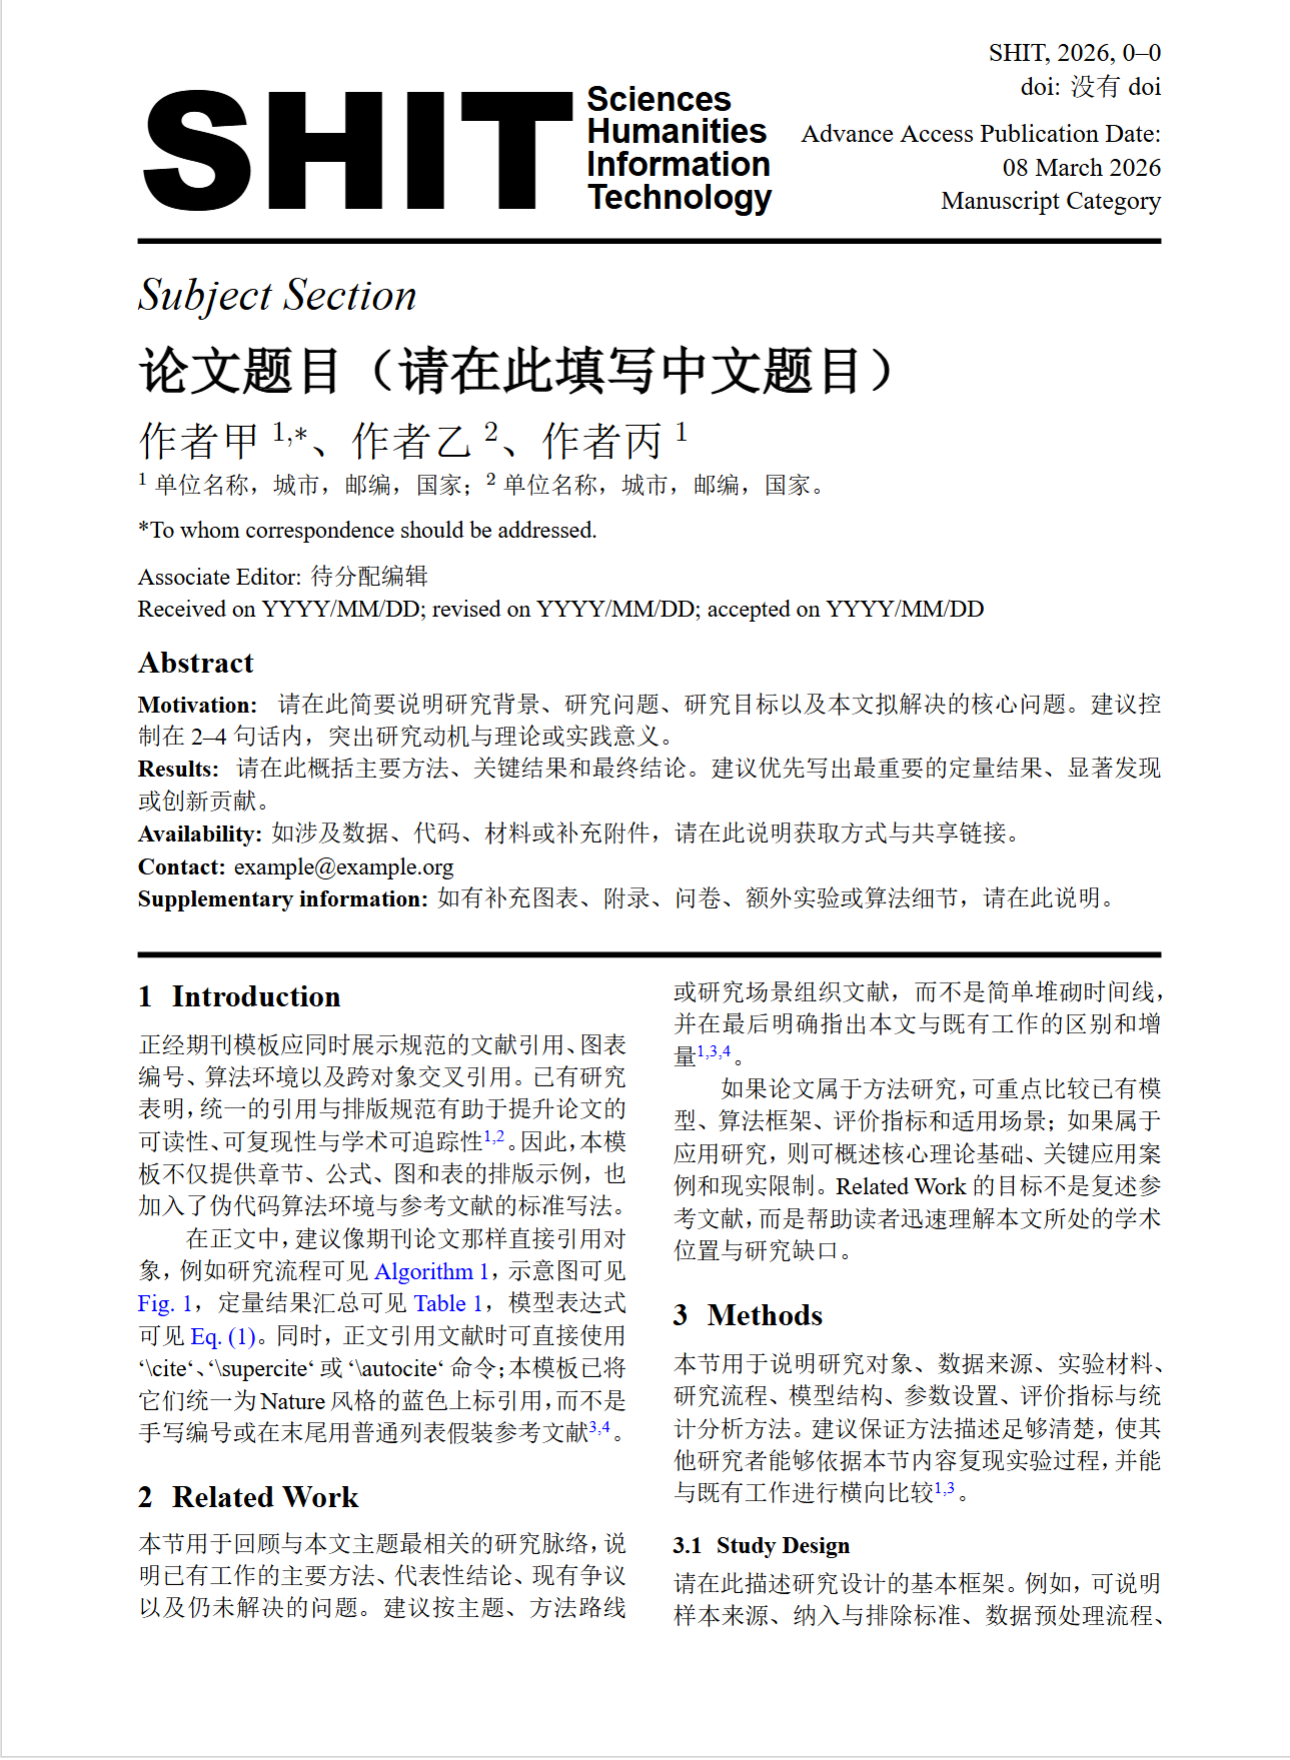
\includegraphics[width=0.96\columnwidth]{SHIT.png}%
}{%
  \fbox{\rule{0pt}{4.2cm}\rule{0.92\columnwidth}{0pt}}%
}
\caption{示例图片标题。可替换为流程图、结果图、结构图或实验示意图。}
\label{fig:workflow}
\end{figure}

\section{Discussion}\label{sec:discussion}
本节用于解释研究结果的意义，比较本研究与已有文献的一致性或差异，分析可能原因，并说明研究的理论价值与应用价值。讨论时可以像期刊论文一样同时回指正文对象，例如“结合 \Cref{alg:pipeline,fig:workflow,tab:metrics} 可见，本研究流程、可视化结果和量化指标之间具有一致性”，并与既有文献进行比较\supercite{ref:article,ref:cnjournal}。若研究存在局限性，例如样本量不足、单中心设计、参数选择有限或外部验证不充分，也建议在本节末尾明确写出。

\section{Conclusion}\label{sec:conclusion}
本节用于概括全文的核心结论、研究贡献与潜在应用前景。建议避免简单重复摘要内容，而是进一步强调本文最重要的发现，并指出未来研究可继续改进的方向。若需要再次引用方法、结果或文献，可继续使用与前文一致的编号体系和交叉引用命令。

\begin{SHITAcknowledgements}
感谢所有参与研究设计、数据整理、实验实施、学术讨论及论文修改的个人或机构。若无致谢内容，可删除本节。
\end{SHITAcknowledgements}

\begin{SHITAIStatement}
\aistatementtext
\end{SHITAIStatement}

\begin{SHITFunding}
请在此填写基金项目名称、项目编号及资助信息。若无基金支持，可写“None”.
\end{SHITFunding}

\noindent\textit{Conflict of Interest:} 作者声明不存在利益冲突。

\printbibliography[title={References}]

\end{document}
